\section{V3}
\subsection{Meiose}

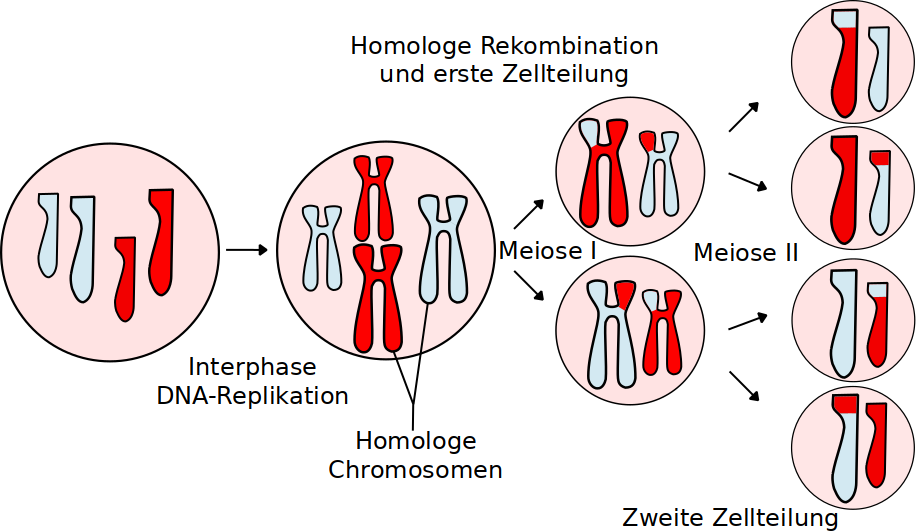
\includegraphics[width=1\textwidth]{lectures/V3/pix/Meiosis_Overview_new.png}

\subsubsection{Zufällige Chromosomenauswahl}
\begin{description}
    \item[Meiose I] Homologe mütterliche und väterliche Chromosomen werden zufällig auf Tochterzellen verteilt
    \item[Meiose II] Chromatiden werden zufällig auf Tochterzellen verteilt
    \item[Mensch] 23 Chromosomen $\Rightarrow 2^{23}~(\approx$ 8 Mio.) Möglichkeiten
\end{description}
\begin{itemize}
    \item Jede Eizelle repräsentiert eine von 8 Mio. Möglichkeiten
    \item Jedes Spermium repräsentiert eine von 8 Mio. Möglichkeiten
    \item Ein Elternpaar produziert eine von 70.368.744.177.644 möglichen Zygoten
    \item Jedes andere Elternpaar aus anderen 70.368.744.177.644 Möglichkeiten
\end{itemize}

\subsection{Mendelsche Gesetze}
\subsubsection{Mendelsche Erbgänge}
\begin{description}
    \item[Dominanter Erbgang] Ein Allel bestimmt die Ausprägung eines Merkmals, auch in heterozygoten Individuen
    \item[Intermediärer Erbgang] Heterozygote Individuen liegen in ihrer Merkmalsausprägung zwischen den Ausprägungen der homozygoten Individuen, pro Zelle beide Merkmale exprimiert
    \item[Kodominanter Erbgang] Beide Merkmale liegen parallel vor (z.B. Sichelzellanämie, A/B Blutgruppen), pro Zelle nur ein Merkmal exprimiert
\end{description}

\subsubsection{Mendelsche Gesetze}
\begin{description}
    \item[1. Mendelsches Gesetz] (Uniformitäts- oder Reziprozitätsgesetz)
        \begin{itemize}
            \item Kreuzt man reinerbige (homozygote) Eltern miteinander, so sind alle direkten Nachkommen (F1-Generation) gleich (uniform)
            \item Es ist egal, welche Merkmalsausprägung vom Vater und welche von der Mutter kommt (Reziprozität)
            \item[] 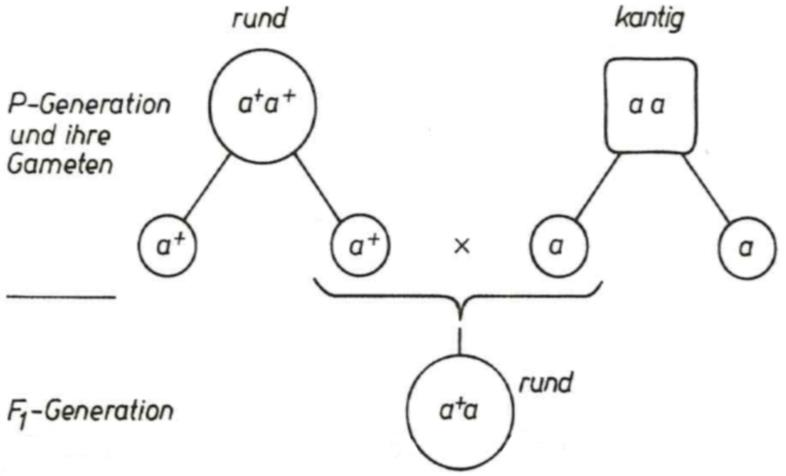
\includegraphics[width=0.5\textwidth]{lectures/V3/pix/Mendel1.jpg}
        \end{itemize}
    \item[2. Mendelsches Gesetz] (Spaltungsgesetz)
        \begin{itemize}
            \item Werden gleichartig heterozygote Organismen gekreuzt, z.B. die F1-Generation aus dem 1. Gesetz, so spalten sich die Allele und die Merkmalsausprägungen wieder auf
            \item Bei einem dominanten Erbgang hat die F2-Generation ein Merkmalsverhältnis von 3 (dominantes Merkmal) : 1 (rezessives Merkmal)
            \item Bei einem intermediären oder kodominaten Erbgang ist das Merkmalsverhältnis 1 : 2 : 1
            \item[] 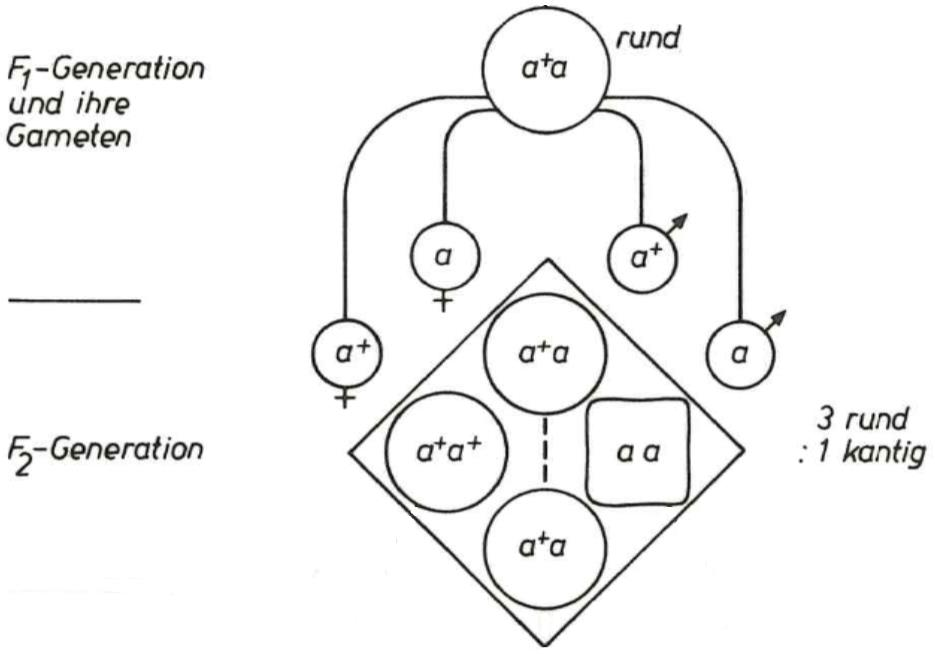
\includegraphics[width=0.5\textwidth]{lectures/V3/pix/Mendel2.jpg}
        \end{itemize}
    \item[3. Mendelsches Gesetz] (Unabhängigkeitsgesetz, Gesetz der Neukombination)
        \begin{itemize}
            \item Bei der Kreuzung von Individuen, die sich in mehreren, durch separate Gene bestimmten Merkmalen unterscheiden, werden diese Merkmale unabhängig voneinander vererbt und frei kombiniert
            \item Dieses Gesetz ist nicht uneingeschränkt gültig siehe (Kopplung, Rekombination)
            \item[] 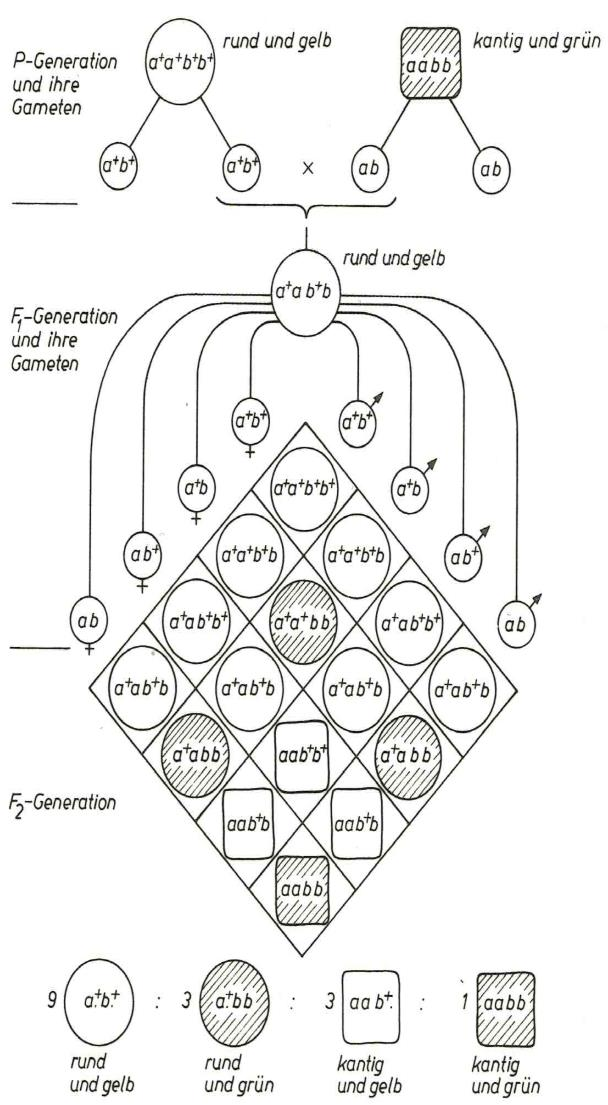
\includegraphics[width=0.5\textwidth]{lectures/V3/pix/Mendel3.jpg}
        \end{itemize}
\end{description}

\subsection{Erbgänge / Stammbäume}

\subsubsection{Segregationsmuster}

\begin{description}
    \item[Autosomal dominant] ~
        \begin{itemize}
            \item Beide Geschlechter gleich betroffen
            \item In jeder Generation sichtbar (insbesondere mindestens ein Elter von Kranken ist betroffen)
            \item Ca. die Hälfte der Kinder Erkrankter ist betroffen
        \end{itemize}
\end{description}
\begin{description}
    \item[Autosomal rezessiv] ~
        \begin{itemize}
            \item Beide Geschlechter gleich betroffen
            \item Nicht in jeder Generation sichtbar, d.h. Eltern Erkrankter können gesund sein
            \item Häufig Familien mit Inzucht
        \end{itemize}
\end{description}
\begin{description}
    \item[X-chromosomal dominant] ~
        \begin{itemize}
            \item Beide Geschlechter betroffen
            \item In jeder Generation sichtbar
            \item Töchter kranker Väter sind sicher betroffen. Söhne gesunder Mütter nicht
            \item 50\% der Töchter/Söhne betroffener Mütter sind betroffen
        \end{itemize}
\end{description}
\begin{description}
    \item[X-chromosomal rezessiv] ~
        \begin{itemize}
            \item Fast nur Männer betroffen
            \item Nicht in jeder Generation sichtbar
            \item Die Töchter von erkrankten Männern sind Anlageträgerinnen
            \item 50\% der Söhne von Anlageträgerinnen sind betroffen, 50\% der Töchter sind wieder Anlageträgerinnen
        \end{itemize}
\end{description}
\begin{description}
    \item[Y-chromosomal] ~
        \begin{itemize}
            \item Nur Männer betroffen
            \item Söhne und Väter Betroffener sind ebenfalls betroffen
        \end{itemize}
\end{description}

\subsection{Gründe für Abweichungen von Mendelschen Erbgängen}
\subsubsection{Genotyp-Phänotyp-Beziehungen}
\begin{itemize}
    \item Sind die genotyischen Varianten ursächlich für phänotypische Ausprägungen?
    \item Maß für den Grad des Zusammenhangs: \textbf{Heritabilität}
    \item Bei komplexen Genotyp-Phänotyp-Beziehungen oft Abweichungen von Mendelschen Gesetzen
\end{itemize}

\subsubsection{Limitierungen der Mendelschen Gesetze}
\begin{itemize}
    \item Unvollständige Penetranz und Phänotypische Plastizität
        \begin{itemize}
            \item Penetranz: Anteil der Individuen mit einem bestimmten Genotyp, die den dazugehörigen Phänotyp ausprägen
            \item Verminderte Penetranz: $P(krank~|~Krankheitsgenotyp) < 1$
            \item Phänotypische Plastizität: Umwelteinflüsse prägen Ausprägung eines Phänotyps
        \end{itemize}
    \item Abweichung bei gonosomalen Erbgängen (X-Inaktivierung)
        \begin{itemize}
            \item Bei Frauen wird das zweite X-Chromosom inaktiviert, um dem Dosisunterschied entgegenzuwirken $\Rightarrow$ Barr-Körperchen
            \item Auswahl beim Menschen zufällig
            \item Verpackung ist vielfältig (Histonmodifikation, DNA-Methylierung)
            \item Verantworktlich: Non-coding-RNA ``Xist''
        \end{itemize}
    \item Phänokopien: Merkmalsausprägung aus anderer Ursache
        \begin{itemize}
            \item Ausprägung eines üblicherweise genetisch bedingten Phänotyps durch Umwelteinflüsse, ohne dass die relevanten genetischen Faktoren vorliegen
            \item $ P(krank~|~normaler ~ Genotyp) > 0 $
        \end{itemize}
    \item Dramatypen: Phänokopie als Reaktion auf akutes Geschehen
        \begin{itemize}
            \item Entstehung eines Phänotyps als akute Reaktion auf sich ändernde Umweltbedingungen
        \end{itemize}
    \item Multiple Allele eines Gens mit verschiedenen phänotypischen Ausprägungen
    \item Multigenische Phänotypen
        \begin{itemize}
            \item Beispiel Hautfarbe: Mendels 2. Gesetz nicht erfüllt
        \end{itemize}
    \item Pleiotropie
        \begin{itemize}
            \item Manche Gene beeinflussen mehrere Phänotypen
        \end{itemize}
    \item Epistasis
        \begin{itemize}
            \item Die Ausprägung eines Gens beeinflusst die Ausprägung eines anderen Gens (Gen-Gen-Interaktion)
            \item Beispiel: Lila Blütenfarbe bei Wicken entsteht nur, wenn für beide Gene jeweils das dominante Allel vorhanden ist
        \end{itemize}
    \item ``Parent of origin''-Effekte
        \begin{itemize}
            \item Effekt einer Mutation auf den Phänotyp hängt davon ab, ob die Mutation von Mutter oder Vater vererbt wurde
        \end{itemize}
\end{itemize}

\subsection{Aufgaben zur Übung 3}
\subsubsection{Aufgabe 1}
\textbf{a.)}
\begin{itemize}
	\item Sensitivität: gibt den Anteil der korrekt als positiv klassifizierten Objekte an der Gesamtheit der tatsächlich positiven Objekte an ($\mathbb{P}(P|K)$)
	\item Spezifität: gibt den Anteil der korrekt als negativ klassifizierten Objekte an der Gesamtheit der in Wirklichkeit negativen Objekte an ($\mathbb{P}(\overline{P}|\overline{K})$)
	\item Prävalenz: welcher Anteil der Menschen einer bestimmten Gruppe (Population) definierter Größe zu einem bestimmten Zeitpunkt an einer bestimmten Krankheit erkrankt ist\\
	Prävalenz=Anzahl der zum Untersuchungszeitpunkt Kranken / Anzahl der in die Untersuchung einbezogenen Individuen
\end{itemize}

\underline{Vierfeldertafel}\\
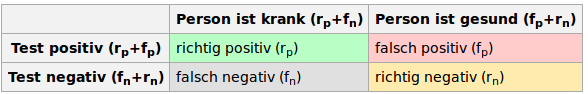
\includegraphics[width=1\textwidth]{lectures/V3/pix/Konfusionsmatrix.png}
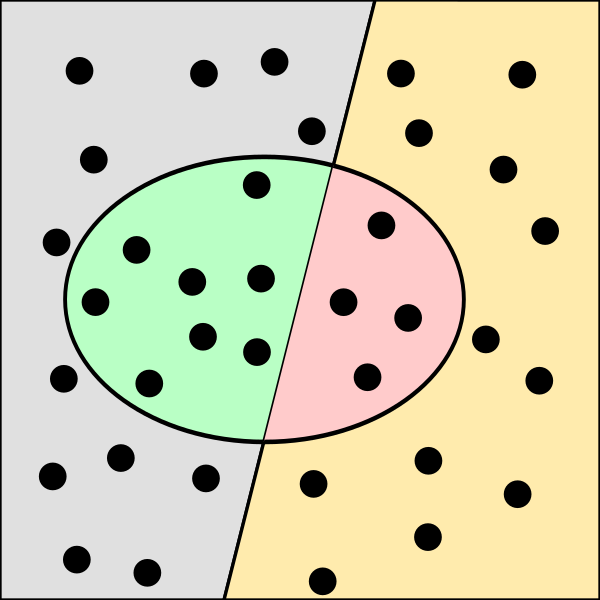
\includegraphics[width=0.5\textwidth]{lectures/V3/pix/Binary-classification-file.png}
\newpage
\textbf{b.)}\\
gegeben:
\begin{itemize}
	\item K=\{Patient ist krank\}
	\item P=\{Test ist positiv\}
	\item Sensitivität: $\mathbb{P}(P|K)=0,95$
	\item Spezifität: $\mathbb{P}(\overline{P}|\overline{K})=0,90$
	\item Prävalenz: $\mathbb{P}(K)=0,1$
\end{itemize}

gesucht:\\
\begin{itemize}
	\item positiv prädiktiver Wert (PPW): \\
	$\mathbb{P}(K|P) = \underbrace{\frac{\mathbb{P}(P|K) \cdot \mathbb{P}(K)}{\mathbb{P}(P)}}_{Satz\ von\ Bayes} = \underbrace{\frac{\mathbb{P}(P|K) \cdot \mathbb{P}(K)}{\underbrace{\mathbb{P}(P|\overline{K})}_{=1-\mathbb{P}(\overline{P}|\overline{K})} \cdot \mathbb{P}(\overline{K}) + \mathbb{P}(P|K) \cdot \mathbb{P}(K)}}_{totale\ Wahrscheinlichkeit}$\\
	$\mathbb{P}(K|P) = \frac{0,95 \cdot 0,1}{0,1 \cdot 0,9 + 0,95 \cdot 0,1} = $ \underline{\underline{0,513513514}}
	\item negativ prädiktiver Wert (NPW):\\
	$\mathbb{P}(\overline{K}|\overline{P})= \frac{\mathbb{P}(\overline{P}|\overline{K}) \cdot \mathbb{P}(\overline{K})}{\underbrace{\mathbb{P}(\overline{P})}_{1-\mathbb{P}(P)}} = \frac{\mathbb{P}(\overline{P}|\overline{K}) \cdot \mathbb{P}(\overline{K})}{1 - (\mathbb{P}(P|\overline{K}) \cdot \mathbb{P}(\overline{K}) + \mathbb{P}(P|K) \cdot \mathbb{P}(K))}$\\
	$\mathbb{P}(\overline{K}|\overline{P})= \frac{0,9 \cdot 0,9}{1-(0,1 \cdot 0,9 + 0,95 \cdot 0,1)} =$ \underline{\underline{0,993865031}}
\end{itemize}

\textbf{c.)}
\\
gegeben:
\begin{itemize}
	\item Sensitivität: $\mathbb{P}(P|K)=0,95$
	\item Spezifität: $\mathbb{P}(\overline{P}|\overline{K})=0,90$
	\item Prävalenz: $\mathbb{P}(K)=0,05$
\end{itemize}

gesucht:\\
\begin{itemize}
	\item positiv prädiktiver Wert (PPW)= \underline{\underline{0,$\overline{33}$}}
	\item negativ prädiktiver Wert (NPW)= \underline{\underline{0,997084548104956}}
\end{itemize}

\textbf{d.)}
siehe R-Script

\subsubsection{Aufgabe 2}

\subsubsection{Aufgabe 3}
siehe R-Script
